\documentclass[12pt, oneside]{article}
\usepackage[utf8]{inputenc}
\title{MATH 20C Notes - Week Six}
\author{C-Rin}
\date{October 2019}

\usepackage{natbib}
\usepackage{graphicx}
\usepackage{gensymb}
\usepackage{amsmath}
\usepackage{amssymb}
\usepackage{wrapfig}
\usepackage{diffcoeff}
\usepackage{microtype}

\graphicspath{ {./images/} }

\begin{document}

\maketitle

\section*{Introduction}
Deep 

\begin{figure}[h!]
\centering
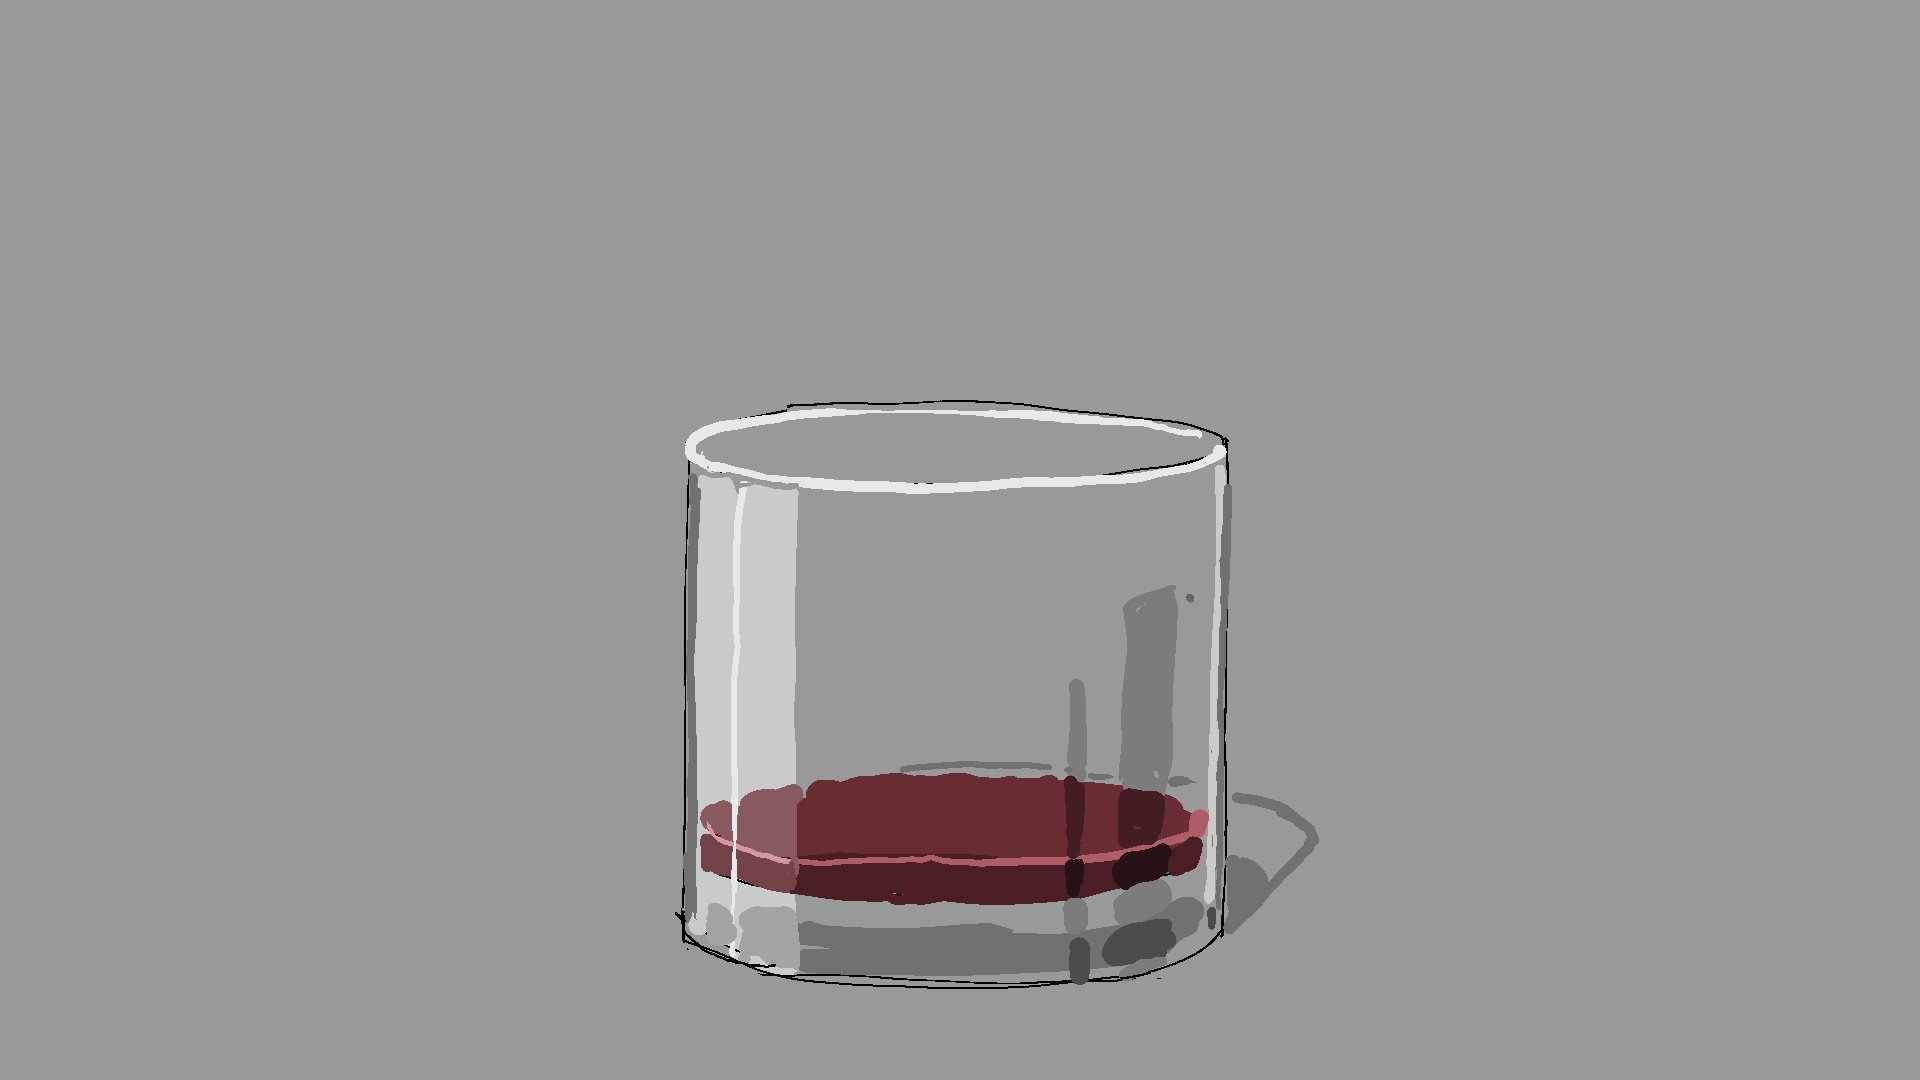
\includegraphics[scale=0.1]{glass.jpg}
\caption{A glass with red liquid (unspecified)}
\end{figure}

\newpage
\section{Double Integrals via Riemann Sums}
\[f:\mathbb{R}^2\rightarrow\mathbb{R}\mbox{ is a continuous function}\]
$[a,b]\times[c,d] = $ \{$(x,y)$ in $\mathbb{R}^2$ so that $a\leq x\leq b$ and $c\leq y \leq d$\}

Goal: Define integral over $[a,b]\times [c,d]$ using riemann sums.
\begin{figure}[h!]
    \centering
    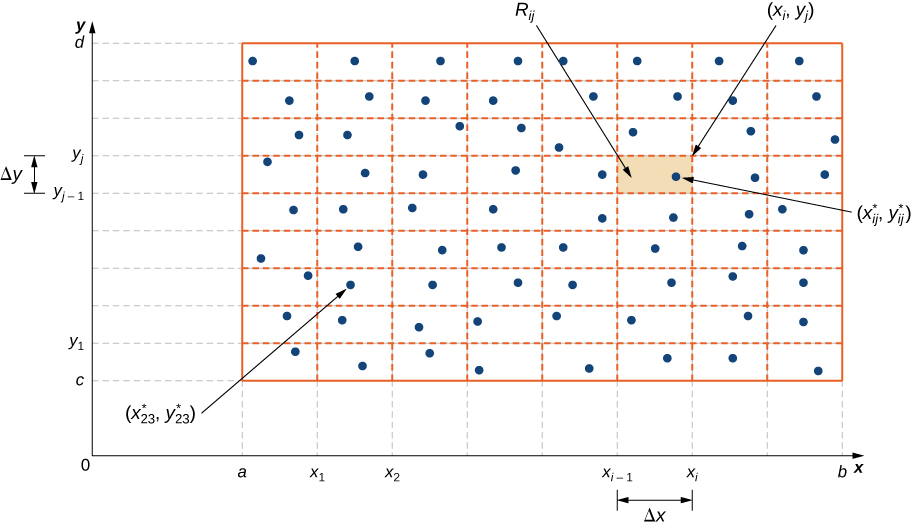
\includegraphics[scale =.5]{nEven.jpg}
    \caption{The region cut into n-even pieces of area $\Delta x\cdot \Delta y$}
    \label{}
\end{figure}

\[\int_n = \sum_{i=1}^{n} \sum_{j=1}^{n} f(x_i , y_i) \Delta y \Delta x\]

\subsection*{Defition}
The double integral of $f(x,y)$ on $[a,b]\times [c,d]$ is $\lim_n\rightarrow\infty \int_n = \int_a^b \int_c^d f(x,y) dydx$.

\subsection*{Remarks}
\begin{enumerate}
    \item If $f$ takes non negative values, then the double integral computes the appropriate values
    \item We do not need $f$ to be continuous to define $\iint (f) dydx$
\end{enumerate}

\textbf{Important Note:} $f$ is integratable if you get the same limit no matter which way you divide $[a,b]\times[c,d]$

\subsection*{Properties of the Integral}
$f(x,y),g(x,y)$ are two continous functions

\subsubsection*{Additively}
\[\int^{b}_{a}\int^{d}_{c} f(x,y) +g(x,y) dydx = \int^{b}_{a}\int^{d}_{c}f(x,y) dydx +\int^{b}_{a}\int^{d}_{c} g(x,y) dydx\]

\subsubsection*{Scaling}
\[\int^{b}_{a}\int^{d}_{c}\lambda f(x,y) dydx = \lambda \int^{b}_{a}\int^{d}_{c} f(x,y) dydx\]
While $\lambda$ is a real number

\subsubsection*{Iteration}
Let $\int^{d}_c f(x,y)dy = A(x)$

\[\int^{b}_{a}\int^{d}_{c} f(x,y)dydx = \int_a^b A(x)dx\]

\subsubsection*{Switching the Order}
\[\int^{b}_{a}\int^{d}_{c} f(x,y)dydx = \int^{d}_{c}\int^{b}_{a} f(x,y) dxdy\]

\subsection*{Excercise}
\[\int^1_0 \int^1_0 x^3+y^2 dydx = \int^1_0 (x^3+y^2) dy = \left[x^3 y +\frac{y^3}{3}\right]^1_0\]
\[=x^3+\frac{1}{3}\]
\[\int^1_0 (x^3+\frac{1}{3})dx = \left[\frac{x^4}{4}+\frac{1}{3}x\right]^1_0 = \frac{1}{4}+\frac{1}{3}=\frac{7}{12}\]

\subsection*{Exercise}
\[\int^1_0\int^1_0 ye^{xy}dydx=\int^1_0\int^1_0 ye^xy dxdy\]
\[\int^1_0 ye^{xy} dx = \left[e^xy\right]^1_{x=0}=e^y-1\]
\[\int^1_0 e^y -1 dy = \left[e^y-y\right]^1_0 = e-1-1+0=e-2\]
\subsection*{Exercise}
\[\int^1_0\int^1_0 \ln ((x+1)(y+1))dydx = \int^1_0\int^1_0 \ln (x+1)+\ln {y+1} dydx\]
\[=\int^1_0\int^1_0\ln (x+1)dydx +\int^1_0\int^1_0 \ln (y+1)dydx\]
\[A(x)=\int^1_0 \ln (y+1)dy =\left[(y+1)\ln (y+1) - (y+1)\right]^1_0 = 2\ln(2)-2 -((-1)(ln(1))-1)\]
\[2\ln(2) -2+1 = 2\ln(2)-1\]
\[\int^1_0\int^1_0 \ln(y+1)dydx = \int^1_0 (2\ln(2)-1)dx=2\ln(2)-1\]

\[2\ln2-1+2\ln2-1=4\ln2 -2\]


\end{document}